\chapter{Spoken Dialogue Systems}
\label{chap:spoken_dialogue_systems}

\lettrine{T}{his} chapter gives an overview of the \aclp{sds} paradigm, including common architectures, different system types, and evaluation methods.
The concept of adaptive \aclp{sds}, which is a core idea in this work, is introduced as well, along with examples of adaptation on different levels.

\pagebreak

%\section{What is a spoken dialogue system?}
%\label{sec:what_is_a_sds}

\todo[inline]{here talk about what is a dialogue, a spoken dialogue, turn, when an interaction becomes a dialogue (is every interaction with a machine is a dialogue system?), etc. can really use the introductions given by Olga in the SDS seminar}

Nowadays, \acfp{sds} are used in various forms in our everyday life.
Giving users all the features of a responsive (sometimes personalized, see \cref{subsec:personal_assistants}) dialogue system with the advantage of using voice to communicate, leaving the hands free to perform any other action, such as driving.\\

In recent years, the market for commercial \acp{va} has rapidly grown.
For example, Microsoft Cortana had 133 million active users in 2016 \citep{Osborne2016why} and Echo Dot was Amazon's best-selling product between 2016 and 2018 \citep{Dickey2017echo}.
Furthermore, \SI{72}{\percent} of people who own a smart speaker say they often use their devices as part of their daily routine \citep{Kleinberg2018ways}.

\todo[inline]{give examples of commercial systems and places where SDSs are used}

\section{Types of spoken dialogue systems}
\label{sec:types_of_sdss}

\todo[inline]{short general introduction explaining the term ``computer-based'' agent as a overarching term for all of the other listed below.}

\begin{table}[tb]
	\centering
	\caption[Types of \aclp{sds}: Task-oriented vs.\ Chatbots]{A comparison of some characteristics in task-oriented \acp{sds} and chatbots.}
	\label{tab:sds_types}
	\begin{tabularx}{\linewidth}{>{\bfseries}lp{.35\linewidth}p{.35\linewidth}}
		\toprule
							& \multicolumn{1}{c}{{\large \textbf{Task-oriented}}} & \multicolumn{1}{c}{{\large \textbf{Chatbots}}} \\
		\vspace{.2cm}
		Goal				& Help the user achieve a specific, pre-defined goal
							& Converse as naturally and continuously as possible \\
		\vspace{.2cm}
		Applications		& \Aclp{pa}, \ac{cnc} systems, integrated voice-activated systems for cars, reservations, etc.
							& Free-form \acl{c-ai} applications: chit-chat bots, social robots \\
		\vspace{.2cm}
		Domain				& Domain-specific, possibly multi-domain
							& Aim to be domain-free (a.k.a.\ open domain) \\
		\vspace{.2cm}
		Modeling			& Statistical models and/or handcrafted rules
							& Typically \ac{s2s} models with no-go filters \\
		\vspace{.2cm}
		Evaluation			& Task completion rate and completion time, number of turns (+ subjective criteria)
							& Chat length, relevant replies ratio, user engagement, general user satisfaction \\
		\bottomrule
	\end{tabularx}
\end{table}

\subsection{Personal assistants}
\label{subsec:personal_assistants}

\Acp{pa}\ldots

A big advantage of \acp{va} is their simple operation.
Using nothing but speech commands, users can perform tasks like playing music, searching the web, shopping online, etc.
In the future, we are likely to witness an ever-growing presence of devices with spoken interaction capabilities, like speech-activated cars, hands-free medical assistants, and intelligent tutoring systems.
This will increase the demands on voice-activated devices even more, as they will need to support more functionalities in a way that is comfortable and intuitive for the users.
Additionally, it can be expected that such devices will be used not only by individuals, but also in more social contexts, i.e., where multiple humans are involved.


Besides making the operation of such voice-activated systems simple and user-friendly, \acp{pa} also aim to let users interact with them in a familiar, natural manner.
One property of natural interactions is the tendency to accommodate to the specific situation and interlocutors to make the interactions more fluent and efficient \citep{Giles1991CAT,Gallois2015CAT}.
Linguistic accommodation is one aspect of this phenomenon, and it is found in various \ac{hhi} experiments \citep[e.g.,][]{Pardo2017phonetic,Schweitzer2017social}.

\subsection{Intelligent speakers}
\label{subsec:intelligent_speakers}

\Acp{pa} are sometimes integrated into a loudspeaker that can be placed in a central spot at home or in an office\ldots

\subsection{Chatbots and social robots}
\label{subsec:chatbots}

Chatbots (sometimes also called \emph{chatterbots} or \emph{chitchat bots}) are a\ldots

\todo{write a bit about history of chatbots (start with ALICE)}

Chatbots have been used in various domains such as education \citep{Benotti2014engaging, Kerly2007bringing}, culture heritage \citep{Pilato2005expert}, healthcare \citep{Kowatsch2017text}, software development \citep{Lebeuf2017software}, and others \citep{Shawar2007chatbots}.

\subsection{Embodied agents}
\label{subsec:embodied_agents}

\citet{Staum2010virtually, Gijssels2016speech}

\subsection{Virtual agents and virtual humans}
\label{subsec:virtual_agents}

Also known as \textit{avatars}, these...

\section{Architecture of spoken dialogue systems}
\label{sec:architecture_sds}

\todo[inline]{explain that this is a generic, symmetric architecture. there are sometimes some extensions or sub-components to some of the modules}
\todo[inline]{explain that each of the components is a research area by its own}

\begin{figure}[t]
	\centering
	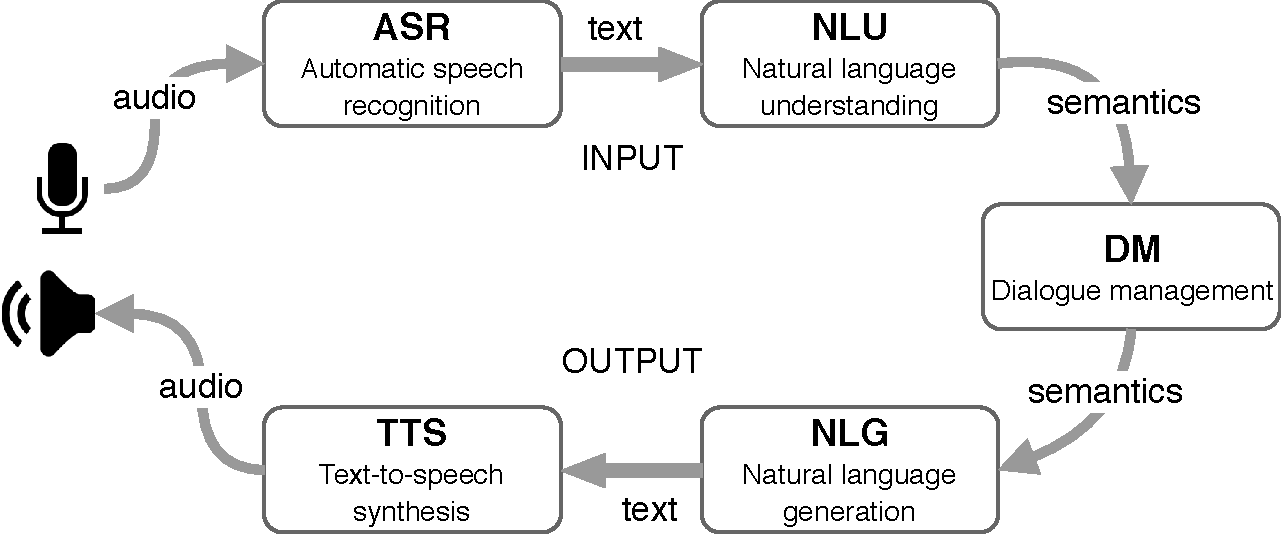
\includegraphics[width=\linewidth]{sds_architecture}
	\caption[Architecture of a spoken dialogue system] {
		A typical architecture of a spoken dialogue system.
		The interaction lifecycle is symmetric, and for each analysis input step there is a corresponding generation output step.
		The exchange usually starts with a user spoken utterance and ends with the system's spoken response.
	}
	\label{fig:sds_architecture}
\end{figure}

Each of a the components shown in \cref{fig:sds_architecture} is a whole research area by itself.
Brief overviews is given here, along with some systems and implementation that can be used for each of these \ac{nlp} task:

\subsection{Automatic speech recognition}
\label{subsec:automatic_speech_recognition}

\subsubsection{Tools}
\label{subsubsec:tools_asr}

\subsection{Natural language understanding}
\label{subsec:natural_language_understanding}

\todo[inline]{be sure to mention the term \enquote{intention}}

\subsubsection{Tools}
\label{subsubsec:tools_nlu}

\subsection{\Acl{dm}}
\label{subsec:dialogue_management}

\todo[inline]{short-mid-length intro to this. about purpose, importance, "core of the SDS", etc.}
\ldots is typically divided into \emph{Belief Tracker} and \emph{Policy}.
\todo[inline]{Now explain about each of them. former is about past turns and anticipating the user's intent, latter is about future responses and what response best matches the user's needs/expectations. mention the use of Reinforcemnet Learning, since it is used when feedback from user is used to improve a system. there are probably papers where this is used.}
\todo[inline]{also explain that this is the part that is connected to external resources, if necessary}

Another component of the \ac{dm} is the \emph{domain}\ldots
Some external knowledge base can be connected as well\ldots
The domain determines what the system can talk about and react to, and to what extent.
\todo[inline]{examples of (simple) domain}
\todo[inline]{combining domains and extending domains, e.g. using crowd sourcing or machine learning}
\todo[inline]{breadth vs.\ depth of domain in SDS (variety vs.\ complexity). replicate the graph Milica showed in her talk (x-axis is breadth and y-axis depth, with some examples along combinations of the axes.)}
\subsubsection{Tools}
\label{subsubsec:tools_dm}

\subsection{Natural language generation}
\label{subsec:natural_language_generation}

\subsubsection{Tools}
\label{subsubsec:tools_nlg}

\subsection{Text-to-speech synthesis}
\label{subsec:text-to-speech_synthesis}

\subsubsection{Tools}
\label{subsubsec:tools_tts}

\section{Accommodative spoken dialogue systems}
\label{sec:adaptive_spoken_dialogue_systems}

Dynamically changing the voice is a capability currently ascribed almost exclusively to humans and exist only sparsely and simplistically in computer-based systems.
A voice-activated device always talks the same way, regardless of how the user speaks to it, the environment and setting in which the interaction takes place, the goal and role of the device, etc.
This capability, which comes naturally to humans in social interactions, involves several steps of (partially unaware) decisions, which together form the overall effect of becoming behaviorally more or less similar to an interlocutor, as explained in \cref{sec:communication_accommodation_theory}.
These include both situational and knowledge-related facets like how it is expected to behave in certain situations and which vocal changes fit those, as well as the physiological ability to apply these matches.
Humans can perform all of these steps as one conduct.
For computers, however, these steps must be broken down and \emph{explained}, as they lack such common social background knowledge and the intuition as for how to match their voice to the situation.
Several attempts to integrate this capability into \acp{sds} are presented below, followed by a description of a roadmap toward such a system and an introduction of relevant terminology to describe these different steps and ways to achieve accommodative vocal behavior in machines.
The parallelisms to the human perspective are highlighted along the way to help understanding the motivations and goals.

Various studies have investigated entrainment and priming in \acp{sds}, aiming to better understand \ac{hci} dynamics and improve task-completion rates.
\citet{Lopes2013automated, Lopes2011primes}, for example, focused on dynamic entrainment and adaptation on the lexical level.
Others, like \citet{Nenkova2008high}, concentrated on word frequency.
\citet{Parent2010lexical} examined changes in both lexical choices and word frequency using the \emph{Let's Go}~\ac{sds} \citep{Raux2005letsgo}.
While these studies addressed the changes in experimental, scripted scenarios, the theoretical foundations for studying these changes in spontaneous dialogue exist as well \citep{Brennan1996lexical}.
\citet{Gasic2013policy, Levin2000stochastic} provide examples of online adaptation for dialogue policies and strategies.
\todo{add 1-2 more sentences for each of the examples?}
Noticeably, while all of the studies mentioned above examine various facets of dialogues, none of those are related to the auditory aspects of speech -- the primary modality used to interact with \acp{sds}.
%Studying convergence in speech in an \ac{hci} context is made possible with more natural synthesis technology, which gives more fine-grained control over parameters of the system's spoken output.
%\todo{need references here?}
There are systems that deal with adaptation of speech-related features focus on prosodic characteristics like intonation or speech rate.
\citet{Levitan2014acoustic} sheds light on acoustic-prosodic entrainment in both \ac{hhi} and \ac{hci} via the use of interactive avatars.
\citet{Bell2003prosodic} found that users' speech rate can be manipulated using a human-simulated \ac{sds}.
Similar results were found when intensity changes in children's interaction with synthesized \ac{tts} output were examined \citep{Coulston2002amplitude}.
A technical overview of the development of adaptive \acp{sds} is given by \citet{Levitan2016implementing}, where speech rate and intensity are manipulated and entrained by the system.

\subsection{Roadmap and challenges}
\label{subsec:roadmap_and_challenges}

The lack of accommodative speech in computer-based systems roots from what is more often than not natural and even automatic for humans, namely realizing how and how much to change their vocal behavior, the physiological means to express those differences, and the ability to combine the two into a coherent production in an interaction.
\Cref{fig:roadmap_adaptive_sds} shows a overview of a (simplified) roadmap to integrating adaptive capabilities into a \ac{sds}.
In addition to of the expected functionalities of a standard \ac{sds}, three main elements are required:
For one thing, knowledge about the nature and properties of accommodative behaviors in humans is required.
This includes both empiric experimental data and integrable models.
% 1-2 sentence that at the moment there are many ways to measure accommodation and existing models are limited (reference? or at least point to terminology part)
Furthermore, the technical capability to control the speech output on demand is essential for introducing flexibility in the system's base voice.
This also includes a mechanism for accumulating phonetic evidence from the user's input relevant for the feature representations used for the accommodation process.
As these manipulations must be applied in real time, re-training the \ac{tts} model to capture every change is not only insufficient, but not practical as well.
This means that the manipulations are done on top of the existing \ac{tts} model, either by modifying the outputted waveform or training a model that can take specific changes in feature description into consideration.
\putref{if chapter about those methods come to life, refer to them}
To link between the modeled theoretical knowledge and the audio processing engineering implementations, an additional component must be introduced in the system.
The role of this component is feed the system's flexible voice parameters result from the models to express vocal changes, which are ultimately conveyed to the user.
This emphasizes the notion of the \ac{nlg} module decides \emph{what} the system says while the \ac{tts} module determines \emph{how} it will say it.
This is further explained and illustrated in \cref{chap:convergence_module_for_sdss,fig:adaptation_module_architecture}.

This work addresses to each of those facets.
\putref{when parts are more final, briefly refer to them here}
These aspects make the task of integrating flexible vocal characteristics into \acp{sds} an involved task, each with its own challenges that requires a profound work to investigate.
%
\begin{figure}[t]
	\centering
	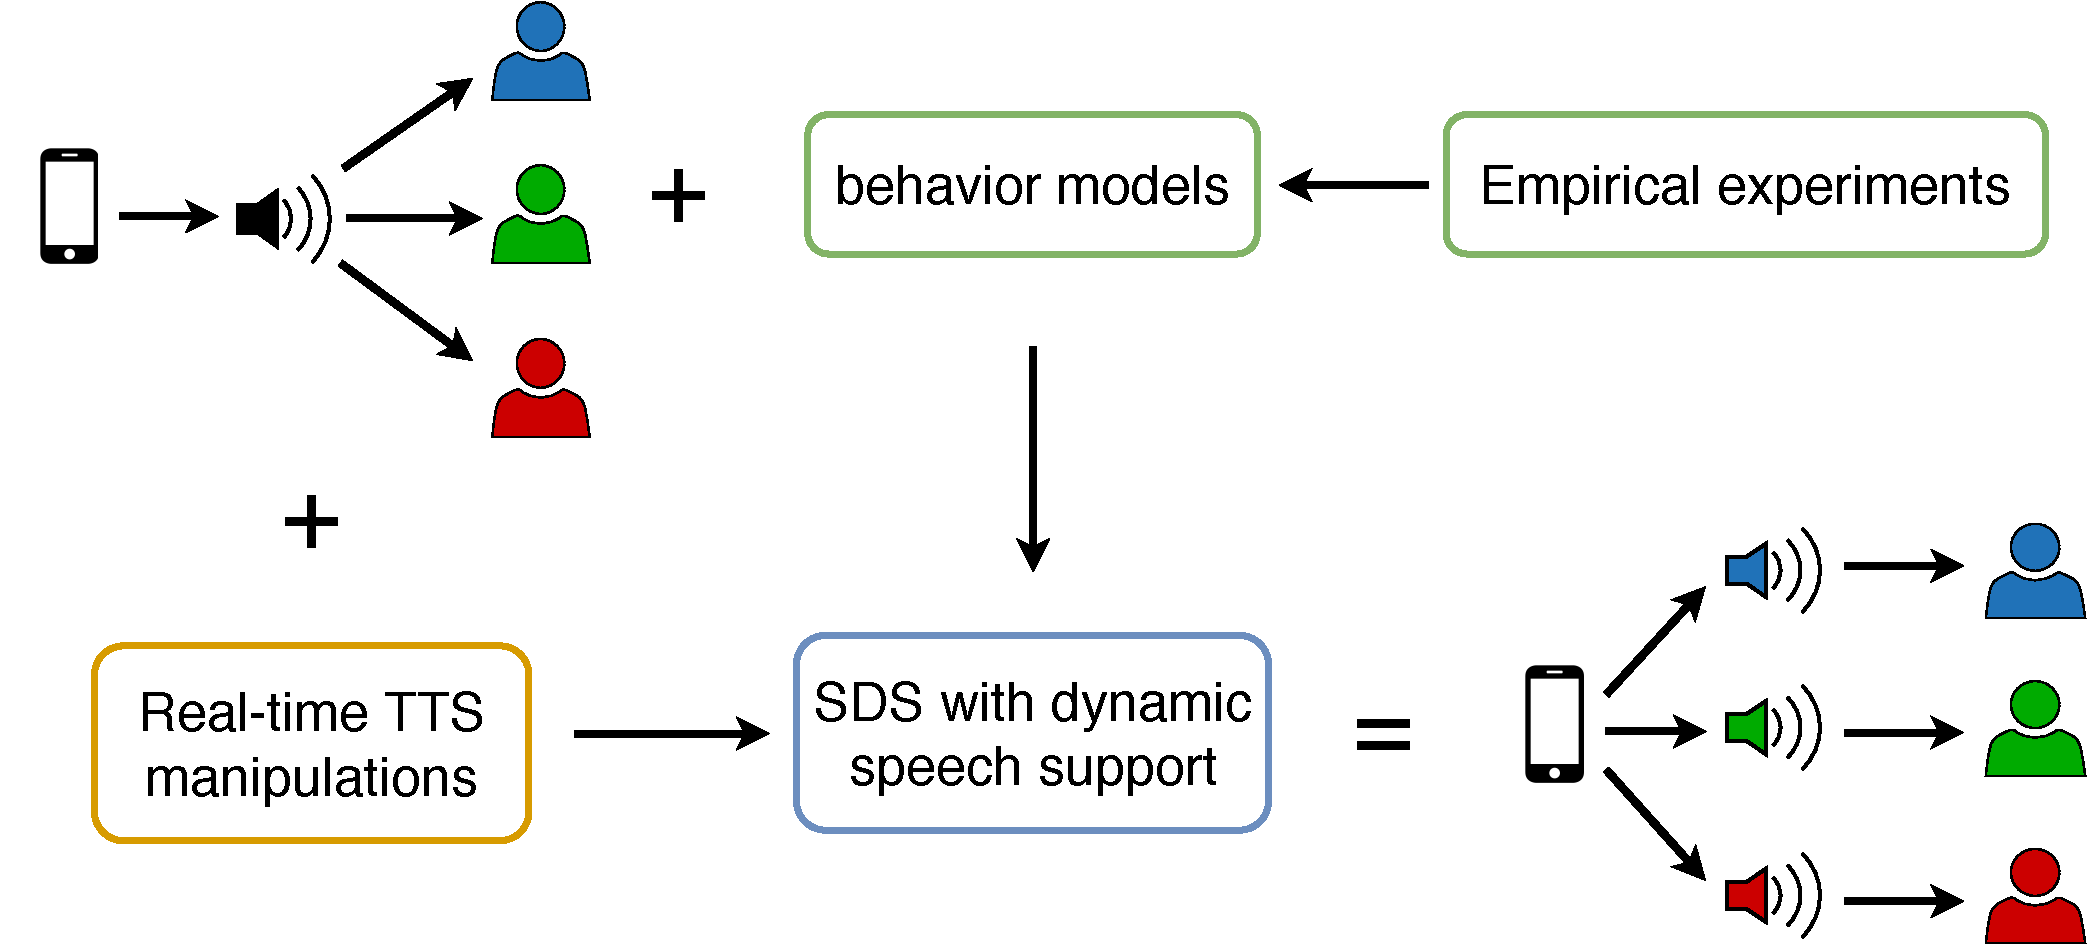
\includegraphics[width=\linewidth]{roadmap_adaptive_sds}
	\caption[Roadmap to phonetically adaptive \acl{sds}]
		{A suggested roadmap from static output (top left) to personalized output (bottom right) in \acp{sds} (and see \cref{fig:output_not_adapted,fig:output_adapted}).
		The green, orange, and blue blocks stand for the modeling, manipulation, and integration components described in the text, respectively.
		The \enquote*{+} signs represents direct addition to a static system and the arrows go from components required as a feed to others.}
	\label{fig:roadmap_adaptive_sds}
\end{figure}
%
For a \ac{sds} to accommodate with its speech, it would not only need to support dynamic, on-demand changes of its \ac{tts} component's output, but would also need its \ac{asr} component to be able to identify and track specific features in the user's speech to update its representation of those features.
Completing the cycle, these representation can then be used as additional input for the \ac{tts} components to determine how those would influence the system's speech output.
This process is individual for each speaker (see \cref{fig:static_vs_adaptive_speech_output}) and may occur over long period of times or multiple interactions, depending of the desired degree and characteristics of accommodation.
Furthermore, this process may involve other component of the \ac{sds} as well (cf.\ \cref{fig:sds_architecture}).
For instance, the Dialogue Manager might consider changes in the user's speech when making decisions, e.g., based on apparent mood and calmness.
The \ac{nlg} component could make alterations to its output to better fit the vocal changes of the system and the user's dynamic state, such as shortening sentences and omit additional information if phonetic indicators of hurry or urgency (like those shown by \citet{Edworthy2003acoustic}) are detected in the speech input.

\subsection{Terminology -- accommodation levels}
\label{subsec:accommodation_levels}

In addition to all the above, another design choice for accommodative \acp{sds}, which is not explicitly required in human speech, concerns the overall \emph{level of accommodation} the system introduces.
This determines the fundamental behavior and form of variation in the system's speech, regardless of specific phonetic features, utterance contents, etc.
The variation levels (or properties) described below can potentially be combined in different ways to achieve the desired system behavior.
They are, at least to some extent, analogous to aforementioned processes conducted by humans in social interactions, with the key difference that humans don't need to defined and think about them separately, if at all.
The utilization these levels is demonstrated in the context of phonetic accommodation, which is one case of dynamic change of speech \citep[as in][to name a few]{Weise2019individual, Schweitzer2016exemplar, Bevnuvs2014social}.
\Cref{chap:web-based_responsive_spoken_dialogue_system} further discusses and demonstrates the integration of such properties into a \ac{sds}.

Different terms are used in the literature to describe systems that can change their output.
This often leads to inconsistencies and mix-ups in terminology.
Definitions of five core properties of accommodative \ac{tts} that should, once accomplished, grant a more dynamic appearance, along with their suggested use and potential fusion with one another, are suggested below.
These terms seek to distinguish between the different capabilities that can be integrated into \acp{sds} and the way they relate to each other and to humans' behaviors.
%
\begin{description}
	\item[Adaptive] -- the vocal behavior evolves between and/or during interactions.\\
	This property refers to the system's use of any mean to \emph{dynamically} change it speech-related behavior, regardless the source of influence, the goal or direction, or specific realizations.
%	Here, adapting means shifting the overall behaviors by updating a subset of the other properties.
	That means, for example, modifying the base behavior, extending the variability, or reflecting the system's changes earlier.
	This can happen between interactions or withing a single, usually longer, interaction.
	The former could be more useful for \ac{cnc} systems or goal-oriented \acp{sds} that are used by many users, while the latter suits social systems like chatbots better and \acp{pa} (see \cref{sec:types_of_sdss}).
	Ultimately, this is a means for the system to improve its performance and accessibility based on previous interactions.
	However, for some applications, like a \ac{capt} system, for example, it would be better to \enquote{reset} their behavior between each use to offer a better experience.

	\item[Flexible] -- on-demand speech manipulation \emph{without rebuilding the voice}.\\
	This property refers to the \emph{technical capability} to alter the system's speech output on request, which is achieved either via modifications in the voice's representation and parameters or by manipulating the outputted waveform directly using signal processing methods.
	Note that this does not entail the way this capability is used, and especially not that it is applied automatically.
	Moreover, as mentioned above, the technical capability to control the voice alone is not enough to create an accommodative behavior.
	This would also require additional data to be transferred to the \ac{tts} component to determine what manipulation to perform.
	For that end, the modeling steps can be build on top of this technical ground.
	It is important to note that this property compensates for the inherent ability in humans to control their voice at will, and therefore does not directly represents any specific element of humans speech behavior like the other properties.
	
	\item[Responsive] -- changes are influenced by some \emph{external} speech input.\\
	A responsive system can, for instance, detect some target features in the user's speech input and, after comparing them to the system's representation of these features, guide the \ac{tts} how to update them (typically, to make them more similar to the user's input).
	This requires some computational model to perform the these steps (cf.\ \cref{chap:computational_model}).
	Yet this model would not have an independently defined behavior and it could only directly become more similar (or dissimilar) to the user in some fashion.
	Such models can be designed to imitate the user's immediate output from previous turns (like in \citet{Levitan2016implementing}) or to gradually match it based on some parameters like sensitivity and interaction's history (as demonstrated in \citet{Raveh2017Interspeech}).
	This property represents the idea that humans change their speech (and behavior in general) when interacting with other people, which is a key aspect of the \ac{cat} \citep[][and see \cref{sec:communication_accommodation_theory}]{Giles1991CAT}.
	
	\item[Characterized (Profiled)] -- the voice has its own base behavior.\\
	Giving a \enquote{character} (or a \emph{profile}) to a voice means that it has a specified base behavior, which might include general properties of accommodation.
	This can also be seen as a \emph{role} the system plays in a conversation, e.g., if built based on a certain \ac{hhi} scenario \citep{Silber-Varod2018prosodic}.
	In that case, the system would try to stick to some pre-defined model, which contains the required information to fulfill said role.
	A system might also have several profiles to switch between based on the settings and goals of the interaction.
	In the context of accommodation, that would include, for example, the degree of accommodation, its timing, or how strongly the system will try to influence the user's speech.
	This property represents the fact that a human-being has a certain -- however complex -- personality.
	More specifically, a vocal identity, which will be expressed in spoken interactions.
	
	\item[Variable] -- variations on top of the base behavior are yielded.\\
	Some variations can be introduced based on the base profile.
	These are relatively minor differences that deviate from the voice's characteristics or enhance them in some way.
	From a system's point of view, the main purpose of such variations is to make the output style non-deterministic and therefore less repetitive and predictable.
	From the human point of view, this coincides with the difficulty to reproduce identical utterance in exactly the same way every time.
	Moreover, people, though having their own individual personality, would speak differently based on various factors outside a conversation like their mood, the environment conditions, time constraints, etc.
	This property therefore comes to grant some smaller-scale dynamics to the voice, in particular when its base behavior is deterministic.
\end{description}
%

% ----------
% REVIEW: Only mention in case some statistical model is include in the thesis that deals with that (a time-series one or variational autoencoder). in that case briefly say what it means and refer to the relevant chapter

%This work concentrates on facets concerning the properties \emph{characterized} and \emph{variable}, which have been given little attention in \ac{sds} research.
%Together, these two properties results in a flexible, non-deterministic output derived from a defined core behavior (that might itself vary).
%Added to the responsive output creates a system that changes with respect to the user according to its own base behavior and probabilistic variations.
%The balance between the influences from the user input and the system's profile can be defined as well, similarly to the bias utilized in speech adaptation, in the form of \putref{reference to this method)}
%\todo{sentence about balance might be unnecessary}
% ----------

\section{Evaluating spoken dialogue systems}
\label{sec:evaluation_of_sdss}

\ldots Therefore, evaluation of \acp{sds} depends on the purpose of the systems, which can be divided into two types, namely \textit{\aclp{tds}} and \textit{\aclp{ngs}}.

\subsection{Task-driven Systems}
\label{subsec:task-driven_systems}
[doesn't really evaluate the \ac{sds}, but it's ability to predict what task should be performed]
[typically part of a bigger system (which has a set of tasks it can perform (e.g. personal assistant))]

\subsection{Non-goal Systems}
\label{subsec:non-goal_systems}

A \acf{ngs} is a \ac{sds} that does not necessarily aim to complete a specific task (unlike \acp{tds}).
Its purpose is, then, more general and there might not even be a defined purpose for it.
Chatbots (see \cref{subsec:chatbots}) are a good a example for a \ac{sds} that typically isn't used for accomplishing a practical task like getting information or operating a device.
Instead, they are used as a long-term social companion (be it at home or as part of a mobile device) and even merely for entertainment. \todo{references for both examples}
Since such systems don't help achieving a defined goal, it is not possible to evaluate their performance based on how well (or whether at all) this goal task was carried out.
There is a need therefore for another, more long-term and interaction-oriented method rather than a task-oriented method.
On the one hand, from the \ac{hci} point of view, the advantage of such methods is that they evaluate the dialogue capabilities of the system and not merely it's ability to map speech patterns or keywords to a set pre-defined actions.
On the other hand, however, the problem in such methods is that it is much harder to define metrics when the goal of the interaction is not completely defined.
There are two approaches to solve this issue:
The first is defining the 
